%%%%%%%%%%%%%%%%%%%%%%%%%%%%%%%%%%%%%%%%%%%%
%Classe de documento
%%%%%%%%%%%%%%%%%%%%%%%%%%%%%%%%%%%%%%%%%%%%
\documentclass[12pt,openright,twoside,english,brazil]{abntex2} 
%%%%%%%%%%%%%%%%%%%%%%%%%%%%%%%%%%%%%%%%%%% 
%Pacotes de língua 
%%%%%%%%%%%%%%%%%%%%%%%%%%%%%%%%%%%%%%%%%%%
%\usepackage[backend=biber]{biblatex}
\usepackage[utf8]{inputenc}
\usepackage{mathtools}
\usepackage{amsfonts}
\usepackage{mathrsfs}
\usepackage{newtxmath} 
\usepackage{Alegreya}
\usepackage{AlegreyaSans}
\usepackage[lf]{FiraMono}
\usepackage[italic]{mathastext}
\usepackage{microtype} 				% para melhorias de justificação
\usepackage[dvipsnames]{xcolor} 		% para cores
\usepackage{graphicx} 			% para imagens
\usepackage{booktabs,tabularx,rotating}	% para tabelas
\usepackage{mdframed} 				% para caixas de texto como na CIP do verso do título
\usepackage{multicol}				% tabelas com colunas mescladas
\usepackage{lettrine}				% letras capitulares
\usepackage{xspace} 				% para nao precisar de espaços com {} depois de comandos
\usepackage{leading}				% espaçamento entrelinhas
%\leading{13pt}
\usepackage[brazilian,hyperpageref]{backref}	
%\usepackage{hyperref}
\bibliographystyle{plain}
\usepackage{subcaption}
\usepackage[num]{abntex2cite}
% ---
% Configurações do pacote backref
% Usado sem a opção hyperpageref de backref
\renewcommand{\backrefpagesname}{Citado na(s) página(s):~}
% Texto padrão antes do número das páginas
\renewcommand{\backref}{}
% Define os textos da citação
\renewcommand*{\backrefalt}[4]{
	\ifcase #1000 %
		Nenhuma citação no texto.%
	\or
		Citado na página #2.%
	\else
		Citado #1 vezes nas páginas #2.%
	\fi}%
% ---
\usepackage[T1]{fontenc}
\usepackage{textcomp}
\usepackage{listings}
\usepackage{color}
\definecolor{dkgreen}{rgb}{0,0.6,0}
\definecolor{gray}{rgb}{0.5,0.5,0.5}
\definecolor{mauve}{rgb}{0.58,0,0.82}

\lstset{frame=tb,
  language=Python,
  aboveskip=3mm,
  belowskip=3mm,
  showstringspaces=false,
  columns=flexible,
  basicstyle={\small\ttfamily},
  numbers=left,
  numberstyle=\tiny\color{gray},
  keywordstyle=\color{blue},
  commentstyle=\color{dkgreen},
  stringstyle=\color{mauve},
  breaklines=true,
  breakatwhitespace=true,
  tabsize=3
}

\lstset{literate=
  {á}{{\'a}}1 {é}{{\'e}}1 {í}{{\'i}}1 {ó}{{\'o}}1 {ú}{{\'u}}1
  {Á}{{\'A}}1 {É}{{\'E}}1 {Í}{{\'I}}1 {Ó}{{\'O}}1 {Ú}{{\'U}}1
  {à}{{\`a}}1 {è}{{\`e}}1 {ì}{{\`i}}1 {ò}{{\`o}}1 {ù}{{\`u}}1
  {À}{{\`A}}1 {È}{{\'E}}1 {Ì}{{\`I}}1 {Ò}{{\`O}}1 {Ù}{{\`U}}1
  {ä}{{\"a}}1 {ë}{{\"e}}1 {ï}{{\"i}}1 {ö}{{\"o}}1 {ü}{{\"u}}1
  {Ä}{{\"A}}1 {Ë}{{\"E}}1 {Ï}{{\"I}}1 {Ö}{{\"O}}1 {Ü}{{\"U}}1
  {â}{{\^a}}1 {ê}{{\^e}}1 {î}{{\^i}}1 {ô}{{\^o}}1 {û}{{\^u}}1
  {Â}{{\^A}}1 {Ê}{{\^E}}1 {Î}{{\^I}}1 {Ô}{{\^O}}1 {Û}{{\^U}}1
  {ã}{{\~a}}1 {ẽ}{{\~e}}1 {ĩ}{{\~i}}1 {õ}{{\~o}}1 {ũ}{{\~u}}1
  {Ã}{{\~A}}1 {Ẽ}{{\~E}}1 {Ĩ}{{\~I}}1 {Õ}{{\~O}}1 {Ũ}{{\~U}}1
  {œ}{{\oe}}1 {Œ}{{\OE}}1 {æ}{{\ae}}1 {Æ}{{\AE}}1 {ß}{{\ss}}1
  {ű}{{\H{u}}}1 {Ű}{{\H{U}}}1 {ő}{{\H{o}}}1 {Ő}{{\H{O}}}1
  {ç}{{\c c}}1 {Ç}{{\c C}}1 {ø}{{\o}}1 {å}{{\r a}}1 {Å}{{\r A}}1
  {€}{{\euro}}1 {£}{{\pounds}}1 {«}{{\guillemotleft}}1
  {»}{{\guillemotright}}1 {ñ}{{\~n}}1 {Ñ}{{\~N}}1 {¿}{{?`}}1 {¡}{{!`}}1 
}
\renewcommand{\lstlistingname}{Código}
\renewcommand{\lstlistlistingname}{Lista de códigos}
% Configura a ``Lista de Códigos'' conforme as regras da ABNT (para abnTeX2)
\begingroup\makeatletter
\let\newcounter\@gobble\let\setcounter\@gobbletwo
  \globaldefs\@ne \let\c@loldepth\@ne
  \newlistof{listings}{lol}{\lstlistlistingname}
  \newlistentry{lstlisting}{lol}{0}
\endgroup

\renewcommand{\cftlstlistingaftersnum}{\hfill--\hfill}

\let\oldlstlistoflistings\lstlistoflistings
\renewcommand{\lstlistoflistings}{%
   \begingroup%
   \let\oldnumberline\numberline%
   \renewcommand{\numberline}{\lstlistingname\space\oldnumberline}%
   \oldlstlistoflistings%
   \endgroup}
%\usepackage{biblatex}
%\addbibresource{biblio.bib}
%%%%%%%%%%%%%%%%%%%%%%%%%%%%%%%%%%%%%%%%% 
%Comandos especiais relacionados à classe 
%%%%%%%%%%%%%%%%%%%%%%%%%%%%%%%%%%%%%%%% 
\autor{Dr. Sócrates de Oliveira Dantas} 
\titulo{Pêndulo - Soluções Gerais} 
\data{2022}
\preambulo{Este material tem o objetivo de divulgar a utilização e soluções gerais de equações diferenciais envolvendo o movimento do pêndulo simples sob várias condições físicas.}
\local{Juiz de Fora, Minas Gerais}
\instituicao{Grupo de Física da Matéria Condensada \\ Departamento de Física \\ Instituto de Ciências Exatas \\ Universidade Federal de Juiz de Fora \\ \abnTeX\ - versão: 0.1}
% alterando o aspecto da cor azul
\definecolor{blue}{RGB}{41,5,195}

% informações do PDF
\makeatletter
\hypersetup{
     	%pagebackref=true,
		pdftitle={\@title}, 
		pdfauthor={\@author},
    	pdfsubject={\imprimirpreambulo},
	    pdfcreator={LaTeX with abnTeX2},
		pdfkeywords={abnt}{latex}{abntex}{abntex2}{livro}, 
		colorlinks=true,       		% false: boxed links; true: colored links
    	linkcolor=blue,          	% color of internal links
    	citecolor=blue,        		% color of links to bibliography
    	filecolor=magenta,      		% color of file links
		urlcolor=blue,
		bookmarksdepth=4
}
\makeatother

% Estilo de capítulos
% \chapterstyle{pedersen} 
% \chapterstyle{lyhne} 
\chapterstyle{madsen} 
% \chapterstyle{veelo}
% Cabecalho padrao
\makepagestyle{abntbookheadings}
\makeevenhead{abntbookheadings}{\ABNTEXfontereduzida\thepage}{}{\ABNTEXfontereduzida\textit\leftmark}
\makeoddhead{abntbookheadings}{\ABNTEXfontereduzida\textit\rightmark}{}{\ABNTEXfontereduzida\thepage}
\makeheadrule{abntbookheadings}{\textwidth}{\normalrulethickness}

% Cabecalho do inicio do capitulo
\makepagestyle{abntbookchapfirst}
\makeoddhead{abntbookchapfirst}{}{}{}

% Configura layout para elementos textuais
\renewcommand{\textual}{%
  \pagestyle{abntbookheadings}%
  \aliaspagestyle{chapter}{abntbookchapfirst}% customizing chapter pagestyle
  \nouppercaseheads%
  \bookmarksetup{startatroot}% 
}

% Margens do documento 
%% (margens do abntex2 não combinam nem com A5 nem com estilos de capítulo da
% classe memoir.)
\setlrmarginsandblock{2.5cm}{3.5cm}{*}
\setulmarginsandblock{2.5cm}{3.5cm}{*}
\checkandfixthelayout
%\bibliographystyle{abnt-num}
%%%%%%%%%%%%%%%%%%%%%%%%%%%%%%%%%%%%%%%%%% 
%Início do corpo do texto 
%%%%%%%%%%%%%%%%%%%%%%%%%%%%%%%%%%%%%%%%%%% 
\begin{document}
\frenchspacing
% ---
% Capa principal
% ---
\begin{titlingpage}
\phantom{xxx}
\vspace{0.5cm}
\huge
\raggedright
\imprimirautor\\
\vspace{2.5cm}
\Huge 
{\centering
%\includegraphics[scale=0.9]{abntex2-modelo-img-marca.pdf}\\[1cm]
\textit{\textcolor{blue}{\imprimirtitulo}}\\[1cm]
}
\centering 
  %este é um símbolo que só aparecerá com a fonte Minion.
\vfill
\Large
 %este é um símbolo que só aparecerá com a fonte Minion.
\imprimirinstituicao
\end{titlingpage}
%\imprimircapa
\begin{dedicatoria} 
\vspace*{\fill} 
Este trabalho é dedicado aos meus queridos filhos Felipe e Vitória, à minha maravilhosa mulher Patrícia e aos meus netos Lucas, Davi e Helena. 
\vspace*{\fill} 
\end{dedicatoria}
\begin{resumo}
É fato que alguns problemas em Física não possuem soluções que possam ser escritas em termos de funções elementares: o pêndulo simples é um destes problemas. A intenção aqui é o desenvolvimento de uma solução geral para o problema do pêndulo simples. Tradicionalmente, a solução mais simples é a que surge nos livros texto introdutório de Física em cursos de engenharias e ciências exatas. A busca por uma solução geral para o problema do pêndulo simples nos permite avançar em estudos de soluções de equações diferenciais não lineares. Usaremos a abordagem da Lagrangeana para obter a equação diferencial que descreve o comportamento do pêndulo e a seguir exibir alguns resultados e gráficos mostrando seu comportamento para algumas condições iniciais. Utilizamos a linguagem Python para gerar os gráficos mais importantes que nos permitem analisar o comportamento do sistema. Não há novidade, este texto se baseia em trabalhos anteriores que - quando necessário - são citados ao longo do desenvolvimento. A novidade deste texto são os códigos, apesar de serem nossos desenvolvimentos, podem ser copiados e divulgados livremente aos interessados no assunto desde que seja citada a fonte.
\end{resumo}
\tableofcontents* % imprime sumário
\newpage
\begin{KeepFromToc}
\listoffigures
\end{KeepFromToc}
\newpage
% ---
% inserir lista de listings
% ---
\pdfbookmark[0]{\lstlistlistingname}{lol}
\begin{KeepFromToc}
\lstlistoflistings
\end{KeepFromToc}
\cleardoublepage
% ---
\textual
\chapter*[Introdução]{Introdução}
\addcontentsline{toc}{chapter}{INTRODUÇÃO}
\lettrine[nindent=0.35em,lhang=0.40,loversize=0.3]{E}{m} primeiro lugar vamos abordar o tema do software que utilizaremos ao longo do texto. A linguagem de programação que utilizaremos é o \href{https://www.python.org}{Python}, que é uma linguagem interpretada mas possui um grande número de módulos que facilitam gerar dados e fazer gráficos para sua análise. Além do que o Python está disponível para todos os sistemas operacionais mais utilizados (Windows, Linux e MacOS). Nosso objetivo não é ensinar como programar em Python, mas como utilizar esta linguagem de programação para atingir nossos objetivos neste livro. Contudo, se um professor quiser utilizar este material para, também, ensinar a linguagem é possível fazê-lo. Importante ressaltar que, se o  leitor quiser utilizar outras ferramentas de programação a lógica presente nos códigos pode ser, sem sombra de dúvida, ainda utilizada desde que com adaptações.

Em particular, o ambiente de programação \href{https://www.anaconda.com}{Anaconda} é uma das plataformas de utilização em Python mais popular. Este ambiente de programação possui a maioria das ferramentas necessárias para o desenvolvimento desde simples códigos até a grandes estruturas para tratamento e análise de dados extremamente complexos. Sua instalação em sistemas operacionais tipo Linux, por exemplo Ubuntu 20.04, obedece ao seguinte conjunto de ações:
\begin{enumerate}
 \item Comece pela atualização do gerenciador de pacotes local. Por exemplo, em uma janela de terminal, utilizando a linha de comando: 
 \begin{verbatim}
  > sudo apt-get update  
 \end{verbatim}
 \vspace{-1.0cm}
 \item Após acessar o site \url{https://www.anaconda.com/}, baixar a versão mais atual do Anaconda para o sistema operacional utilizado;
 \item Execute o arquivo baixado utilizando, por exemplo:
 \begin{verbatim}
  > bash Anaconda3-2021.1.1-Linux-x86_64.sh
 \end{verbatim}
 \vspace{-1.0cm}
 \item De vez em quando é importante atualizar o Anaconda utilizando o seguinte comando:
 \begin{verbatim}
  > conda update conda
 \end{verbatim}
 \vspace{-1.0cm}
\end{enumerate}

Os módulos do Python empregados no desenvolvimento dos códigos presentes neste livro são: \href{hhtps://numpy.org}{NumPy}, \href{hhtps://scipy.org}{SciPy} e \href{https://matplotlib.org}{Matplotlib}.

\chapter[O pêndulo simples]{O pêndulo simples}
\lettrine[nindent=0.35em,lhang=0.40,loversize=0.3]{V}{amos} considerar a representação abaixo, figura \ref{Figura1}, para o nosso pêndulo simples. Esta figura mostra uma visão esquemática do pêndulo simples sob a ação da gravidade ($\vec{g}$) na vertical.  

\begin{figure}[h]
\begin{center}
 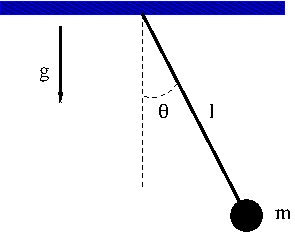
\includegraphics[scale=0.5]{pendulo.png}
\end{center}
\caption{Representação do pêndulo simples.}
\label{Figura1}
\end{figure}

Na figura, $\theta$ é o ângulo entre o pêndulo e a vertical, $l$ o  comprimento do fio e $m$ é a massa do pêndulo. O fio, inextensível e de massa desprezível, vincula a massa a mover-se num plano vertical.

Se utilizarmos $\theta$ e $r$ - as coordenadas polares - como as coordenadas generalizadas, a Lagrangeana é escrita da seguinte forma:
\begin{eqnarray}
L = K - U & = & \frac{1}{2}m \left[ (\dot{r})^2 + (r\, \dot{\theta})^2 \right] - mgr[1-\cos{(\theta)}], \nonumber \\
L & = & \frac{1}{2} m(l\, \dot{\theta})^2 - mgl [1 - \cos{(\theta)} ].
 \label{equa1}
\end{eqnarray}
quando consideramos $r=l$ e a posição inferior do pêndulo ($\theta=0$) como origem do potencial gravitacional: $U(\theta=0)=0$.

Portanto, poderemos escrever a equação de Euler-Lagrange da seguinte forma:
\begin{equation}
 \frac{d}{dt} \left( \frac{\partial L}{\partial \dot{\theta}} \right) - \frac{\partial L}{\partial \theta} = 0,
 \label{equa2}
\end{equation}
onde:
\begin{eqnarray}
 \frac{\partial L}{\partial \dot{\theta}} = ml^2 \dot{\theta} \rightarrow \frac{d}{dt} \left( \frac{\partial L}{\partial \dot{\theta}} \right) = ml^2 \ddot{\theta}, \nonumber
\end{eqnarray}
e
\begin{eqnarray}
 \frac{\partial L}{\partial \theta} = -mgl\sin{(\theta)}, \nonumber
\end{eqnarray}
assim a equação (\ref{equa2}) pode ser reescrita na forma:
\begin{eqnarray}
 ml^2 \ddot{\theta} + mgl \sin{(\theta)} = 0 \rightarrow \ddot{\theta} + \frac{g}{l} \sin{(\theta)} = 0.
 \label{equa3}
\end{eqnarray}

A equação (\ref{equa3}) é uma equação diferencial não linear no tempo. A não linearidade decorre da presença da função seno, o que traz dificuldade na obtenção da solução envolvendo funções elementares. Contudo, nas situações onde $\sin{(\theta)} \approx \theta$, ou seja pequenas oscilações a equação (\ref{equa3}) se torna:
\begin{eqnarray}
 \ddot{\theta} + \frac{g}{l} \theta = \ddot{\theta} + w_0^2 \theta = 0,
 \label{equa4}
\end{eqnarray}
com $w_0=\sqrt{\frac{g}{l}}$ sendo a frequência de oscilação do pêndulo neste limite.

A solução para a equação diferencial (\ref{equa4}) é da forma:
\begin{eqnarray}
 \theta (t) =  A \cos{(w_0t+\phi)}.
 \label{equa5}
\end{eqnarray}
Agora, se considerarmos as seguintes condições iniciais:
\begin{eqnarray}
 \theta(t=0) & = & \theta_0 \nonumber \\
 0 \leq & \theta_0 & \leq \pi \\
 \left( \frac{d \theta}{dt} \right)_{t=0} & = 0, \nonumber
 \label{equa6}
\end{eqnarray}
teremos:
\begin{eqnarray}
 \theta(t) = \theta_0 \cos{(w_0t)}.
 \label{equa7}
\end{eqnarray}
Assim, as oscilações periódicas possuem amplitude $\theta_0$, frequência $w_0=\sqrt{\frac{g}{l}}$, consequentemente o período de cada oscilação é:
\begin{eqnarray}
 T = 2\pi \sqrt{\frac{l}{g}},
 \label{equa8}
\end{eqnarray}
que é independente de $\theta_0$.


\section{Estabilidade}
Levando em consideração a equação (\ref{equa3}) se definirmos: $\theta = x$ e $\frac{d\theta}{dt} = y$ é possível termos o seguinte sistema de equações diferenciais:
\begin{equation}
 \left\{
     \begin{array}{lr}
       \dot{x} = y \\
       \dot{y} = - w_0^2 \sin{(x)}
     \end{array}
     \right.
 \label{equa9}   
\end{equation}

Para encontrar os pontos de equilíbrio do sistema (\ref{equa9}), fazemos:
\begin{equation}
 \left\{
     \begin{array}{lr}
       y = 0 \\
       - w_0^2 \sin{(x)} = 0
     \end{array}
     \right.
 \label{equa10}   
\end{equation}
que nos leva a $x=\pm n \pi$, com $n=0,1,2,...$ e $y=0$, assim os pontos de equilíbrio de (\ref{equa9}) são $ (\pm n \pi,0) $ com $n=0,1,2,3,...$. Esses pontos correspondem a duas posições fixas de equilíbrio. O primeiro caso é quando $n$ é par a massa do pêndulo está abaixo do suporte (na posição mais baixa). O segundo caso é quando $n$ é ímpar e a massa está posicionada acima do suporte, na posição mais alta. Estas situações estão ilustradas na figura \ref{Figura2}.

\begin{figure}[h]
 \begin{center}    
  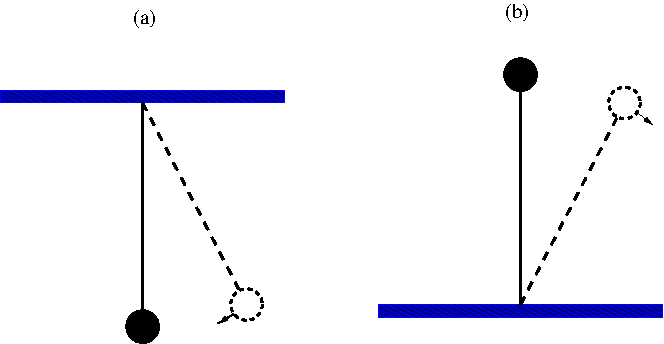
\includegraphics[scale=0.5]{pendulo-2.png}
 \end{center}
 \caption{Representações de equilíbrio: (a) pêndulo em sua posição mais baixa, onde $n$ é par; (b) pêndulo em sua posição mais alta, onde $n$ é ímpar.}
 \label{Figura2}
\end{figure}

Analisando as imagens na figura \ref{Figura2} é quase que intuitivo perceber que a situação (a) é a de equilíbrio estável e a (b) de equilíbrio instável. Na configuração (a) se a massa for deslocada ligeiramente de sua posição de equilíbrio ela irá oscilar indefinidamente com amplitude fixa em torno do ponto mais inferior. Por outro lado, na configuração (b) qualquer ligeiro deslocamento fará com que a massa se desloque para baixo sob influência da gravidade.

Existe uma abordagem matemática para interpretar o comportamento do pêndulo nestes dois pontos críticos: analisando o sistema de equações diferenciais (\ref{equa9}) nestes pontos:
\begin{enumerate}[label=\alph*)]
 \item Vamos analisar como podemos escrever as equações (\ref{equa9}) no ponto inferior (figura 2(a)) quando $\sin{(x)} \approx x$ teremos:
\begin{eqnarray}
 \begin{bmatrix}
 \frac{dx}{dt} \\
 \frac{dy}{dt}
 \end{bmatrix}
 = \begin{bmatrix}
    0 & 1 \\
    -w_0^2 & 0
   \end{bmatrix}
   \begin{bmatrix}
    x \\
    y
   \end{bmatrix},
\end{eqnarray}
o polinômio característico é: 
\begin{equation}
 \lambda^2 + w_0^2=0, \nonumber
\end{equation}
cujos autovalores e respectivos autovetores são: 
\begin{itemize}
 \item para $\lambda_{+} = i\, w_0$ teremos:
      \begin{eqnarray}
       V_{+} = \begin{bmatrix}
                1 \\
                i\, w_0
               \end{bmatrix},
      \end{eqnarray}
 \item para $\lambda_{-} = -i\, w_0$ teremos:
      \begin{eqnarray}
       V_{-} = \begin{bmatrix}
                1 \\
                -i\, w_0
               \end{bmatrix},
      \end{eqnarray}
 \item é fácil observar que $V_{-} = V_{+}^{*}$, ou seja um é o conjugado do outro.        
\end{itemize}

Consequentemente a solução geral é:
\begin{eqnarray}
 X & = & k_1 e^{\lambda_{+}t} V_{+} + k_2 e^{\lambda_{-}t} V_{-} \nonumber \\
   & = & k_1 e^{iw_0t} V_{+} + k_2 e^{-iw_0t} V_{-} \nonumber \\
   & = & k_1 e^{iw_0t} V_{+} + k_2 \left( e^{iw_0t} V_{+} \right)^{*},
\end{eqnarray}
assim:
\begin{eqnarray}
 e^{iwt}V_{+} & = & \begin{bmatrix}
                 \cos{(w_0t)} + i\, \sin{(w_0t)} \\
                i\, w_0\cos{(w_0t)} - w_0 \sin{(w_0t)}
                \end{bmatrix} \nonumber \\
              & = & \begin{bmatrix}
                     \cos{(w_0t)} \\
                     -w_0 \sin{(w_0t)}
                    \end{bmatrix} + i \begin{bmatrix}
                                       \sin{(w_0t)} \\
                                       w_0 \cos{(w_0t)}
                                      \end{bmatrix} \nonumber \\
              & = & V_{1} + i \, \, V_{2},
\end{eqnarray}
com:
\begin{eqnarray}
 V_1 = \begin{bmatrix}
        \cos{(w_0t)} \\
        -w_0 \sin{(w_0t)}
       \end{bmatrix}, \nonumber
\end{eqnarray}
e:
\begin{eqnarray}
 V_2 = \begin{bmatrix}
        \sin{(w_0t)} \\
        w_0 \cos{(w_0t)}
       \end{bmatrix}, \nonumber
\end{eqnarray}
perceba que o termo inferior tanto de $V_1$ quanto $V_2$ é a derivada do termo superior. Logo, a solução geral pode ser reescrita como:
\begin{eqnarray}
 X & = & k_1 (V_1 + i\, \, V_2) + k_2 (V_1 - i\, \, V_2) \nonumber \\
   & = & (k_1 + k_2) V_1 + i (k_1 - k_2) V_2.
\end{eqnarray}
Uma vez que a solução que estamos procurando deve ser real é claro que $k_1=k_2$, assim:
\begin{eqnarray}
 X = 2k_1 V_1 = k\, V_1,
\end{eqnarray}
mantendo somente a primeira componente de $V_1$, teremos como solução:
\begin{eqnarray}
 \boxed{x = \theta (t) = \theta_0 \cos{(w_0t)}},
 \label{equa18}
\end{eqnarray}
considerando a condição inicial que para $t=0 \rightarrow \theta = \theta_0$, teremos $k = \theta_0$. Uma vez que a função oscila no tempo ao com amplitude $\theta_0$, somos levados a admitir que este é um ponto de estabilidade do sistema.

Assim, os pontos $(n\pi,0)$ com $n$ \textbf{par} \textit{são todos pontos críticos estáveis}.

\item Num ponto $x$ próximo ao máximo ($\pi$) escrevendo $u=x-\pi$ e $v=y$, teremos a seguinte expressão diferencial para as expressões (\ref{equa9}):
\begin{eqnarray}
 \begin{bmatrix}
 \frac{du}{dt} \\
 \frac{dv}{dt}
 \end{bmatrix}
 = \begin{bmatrix}
    0 & 1 \\
    w_0^2 & 0
   \end{bmatrix}
   \begin{bmatrix}
    u \\
    v
   \end{bmatrix},
\end{eqnarray}
uma vez que:
\begin{equation}
 \sin{(u)}=\sin{(x-\pi)}\approx -(x-\pi) = -u. \nonumber
\end{equation}

O polinômio característico é: 
\begin{equation}
 \lambda^2 - w_0^2=0, \nonumber
\end{equation}
cujos autovalores e respectivos autovetores são:
\begin{itemize}
 \item para $\lambda_{+} = w_0$ teremos:
      \begin{eqnarray}
       V_{+} = \begin{bmatrix}
                1 \\
                w_0
               \end{bmatrix},
      \end{eqnarray}
 \item para $\lambda_{-} = - w_0$ teremos:
      \begin{eqnarray}
       V_{-} = \begin{bmatrix}
                1 \\
                - w_0
               \end{bmatrix},
      \end{eqnarray}
\end{itemize}
Consequentemente a solução geral é:
\begin{eqnarray}
 U & = & k_1 e^{\lambda_{+}t} V_{+} + k_2 e^{\lambda_{-}t} V_{-} \nonumber \\
   & = & k_1 e^{w_0t} V_{+} + k_2 e^{-w_0t} V_{-} \nonumber \\
   & = & \begin{bmatrix}
          k_1 e^{w_0t} + k_2 e^{-w_0t} \\
          w_0 \, \left( k_1 e^{w_0t} - k_2 e^{-w_0t} \right)
         \end{bmatrix},
\end{eqnarray}
para que tenhamos soluções reais é necessário que $k_1$ e $k_2$ sejam reais e, no sentido de simplificar a análise, na hipótese de serem iguais teremos:
\begin{eqnarray}
 U = 2\, k_1 \begin{bmatrix}
              \cosh{(w_0t)} \\
              w_0 \, \sinh{(w_0t)}
             \end{bmatrix}.
\end{eqnarray}
Mantendo a primeira componente, e suponto que em $t=0$ temos $u=u_0$:
\begin{eqnarray}
 \boxed{u(t) = 2k_1 \cosh{(w_0t)} = u_0 \cosh{(w_0t)}}.
 \label{equa24}
\end{eqnarray}
É fácil observar que esta função diverge quando $t$ cresce. Assim, somos levados a admitir que este ponto é instável. O mesmo ocorre para qualquer ponto $(n\pi,0)$ quando $n$ é \textbf{ímpar}.
\end{enumerate}

\section{Solução exata para velocidade inicial nula}
Vamos nos basear no desenvolvimento efetuado em \cite{bcmbn} para o estudo do pêndulo não linear que conduziu à expressão (\ref{equa3}). Assim, vamos começar reescrevendo a expressão (\ref{equa3}) da seguinte forma:
\begin{eqnarray}
 \frac{d^2 \theta}{dt^2} + w_0^2 \sin{(\theta)} = 0,
 \label{equa25}
\end{eqnarray}
multiplicando a expressão acima por $\frac{d\theta}{dt}$, teremos:
\begin{eqnarray}
 \frac{d\theta}{dt} \frac{d^2 \theta}{dt^2} + w_0^2 \sin{(\theta)} \frac{d\theta}{dt} = 0.
 \label{equa26}
\end{eqnarray}
Que pode ser reescrita como:
\begin{eqnarray}
 \frac{d}{dt} \left[ \frac{1}{2} \left( \frac{d \theta}{dt} \right)^2 - w_0^2 \cos{(\theta)} \right]= 0.
 \label{equa27}
\end{eqnarray}

Utilizando as condições de iniciais (\ref{equa6}) e integrando (\ref{equa27}), encontramos:
\begin{eqnarray}
 \left( \frac{d\theta}{dt} \right)^2 = 2w_0^2 \left[ \cos{(\theta)} - \cos{(\theta_0)} \right].
 \label{equa28}   
\end{eqnarray}
Se utilizarmos a relação trigonométrica:
\begin{eqnarray}
 \cos{(\alpha)} = 1 - 2 \sin^2{\left( \frac{\alpha}{2} \right)}, \nonumber
\end{eqnarray}
reescrevemos a expressão (\ref{equa28}) da seguinte forma:
\begin{eqnarray}
 \left( \frac{d\theta}{dt} \right)^2 = 4w_0^2 \left[ \sin^2{\left( \frac{\theta_0}{2}\right)} - \sin^2{\left( \frac{\theta}{2} \right)} \right].
 \label{equa29}
\end{eqnarray}

Fazendo uma mudança de variáveis:
\begin{equation}
 y = \sin{\left( \frac{\theta}{2}\right)}
 \label{equa30}
\end{equation}
e
\begin{equation}
 k = \sin{\left( \frac{\theta_0}{2}\right)}
 \label{equa31}
\end{equation}
uma vez que $0\leq \theta_0 \leq \pi$ teremos $0\leq k \leq 1$. Levando em consideração as condições iniciais (\ref{equa6}) e as expressões (\ref{equa30}) e (\ref{equa31}) teremos:
\begin{equation}
 y(\theta(0)) = \sin{\left( \frac{\theta(0)}{2} \right)} = \sin{\left( \frac{\theta_0}{2}\right)} = k.
\end{equation}

Derivando (\ref{equa30}) em relação ao tempo teremos:
\begin{equation}
 \frac{dy}{dt} = = \frac{dy}{d\theta} \frac{d\theta}{dt} = \frac{1}{2} \frac{d\theta}{dt} \cos{\left( \frac{\theta}{2} \right)}
\end{equation}
e:
\begin{eqnarray}
 \left( \frac{dy}{dt} \right)^2 & = & \frac{1}{4} \left( \frac{d\theta}  {dt} \right)^2 \cos^2{\left( \frac{\theta}{2} \right)} \nonumber \\
 & = & \frac{1}{4} \left[ 1 - \sin^2{\left( \frac{\theta}{2} \right)}  \right] \left( \frac{d\theta}{dt} \right)^2 \nonumber \\
 & = & \frac{1}{4} \left( 1 - y^2 \right) \left( \frac{d\theta}{dt} \right)^2.
\end{eqnarray}
Ou ainda:
\begin{equation}
 \left( \frac{d\theta}{dt} \right)^2 = \frac{4}{(1-y^2)} \left( \frac{dy}{dt} \right)^2
 \label{equa35}.
\end{equation}
Igualando (\ref{equa35}) a (\ref{equa29}) e lembrando de (\ref{equa30}) e (\ref{equa31}), teremos:
\begin{eqnarray}
 \frac{4}{(1-y^2)} \left( \frac{dy}{dt} \right)^2 & = & 4\, w_0^2 (k^2 - y^2) \rightarrow \nonumber \\
 \left( \frac{dy}{dt} \right)^2 & = & w_0^2 (k^2 - y^2) (1 - y^2) \nonumber \\
 & = & w_0^2\, k^2 \left( 1 - \frac{y^2}{k^2} \right) (1 - y^2) \rightarrow \nonumber \\
 \left( \frac{dy}{d(w_0t)} \right)^2 & = & k^2 \left( 1 - \frac{y^2}{k^2} \right) (1 - y^2),
\end{eqnarray}
fazendo:
\begin{equation}
 \tau = w_0\, t
 \label{equa37}
\end{equation}
encontramos:
\begin{eqnarray}
 \left( \frac{dy}{d\tau} \right)^2 & = & k^2 \left( 1 - \frac{y^2}{k^2} \right) (1 - y^2) \rightarrow \nonumber \\
 \left( \frac{d(y/k)}{d\tau} \right)^2 & = & \left( 1 - \frac{y^2}{k^2} \right) (1 - y^2)
\end{eqnarray}
identificando:
\begin{equation}
 x = \frac{y}{k},
 \label{equa39}
\end{equation}
sendo $x(0)=1$, encontramos a expressão final:
\begin{equation}
 \left( \frac{dx}{d\tau} \right)^2  =  (1 - x^2) (1 - k^2\, x^2)
 \label{equa40}
\end{equation}
sendo:
\begin{equation}
 \left( \frac{dx}{d\tau} \right)_{\tau=0} = 0.
\end{equation}

A expressão (\ref{equa40}) pode ser reescrita como:
\begin{eqnarray}
 \left( \frac{d\tau}{dx} \right)^2  & = & \frac{1}{(1 - x^2) (1 - k^2\, x^2)} \rightarrow \nonumber \\
 d\tau & = & \pm \frac{dx}{\sqrt{(1 - x^2) (1 - k^2\, x^2)}}
 \label{equa41}
\end{eqnarray}
integrando desde $(x(0)=1,dx/d\tau=0)$ até um $(x,dx/d\tau)$ arbitrário na parte inferior do gráfico de $dx/d\tau$ como função de $x$ identifica o intervalo de tempo $\tau$:
\begin{eqnarray}
 \tau & = & -\int_{1}^{x} \frac{dz}{\sqrt{(1 - z^2) (1 - k^2\, z^2)}} \nonumber \\
 \tau & = & \int_{0}^{1} \frac{dz}{\sqrt{(1 - z^2) (1 - k^2\, z^2)}} - \int_{0}^{x} \frac{dz}{\sqrt{(1 - z^2) (1 - k^2\, z^2)}}.
\label{equa43}
\end{eqnarray}
As integrais à direita da última identidade são conhecidas como integrais elípticas de primeira espécie \cite{abramo}, um dos precursores no estudo destas integrais foi Adrien Marie Legendre (1752-1833), entretanto quem ganhou notoriedade neste ramo da matemática foram Niels Hanrik Abel (1802-1829) e Carl Gustav Jakob Jacobi (1804-1851):
\begin{itemize}
 \item completa: \begin{equation}
                  K(k^2) = \int_{0}^{1} \frac{dz}{\sqrt{(1 - z^2) (1 - k^2\, z^2)}},
                 \end{equation}
 \item incompleta: \begin{equation}
                    F(x,k^2) = \int_{0}^{x} \frac{dz}{\sqrt{(1 - z^2) (1 - k^2\, z^2)}}.
                   \end{equation}
\end{itemize}
As expressões acima podem ser escritas em uma forma trigonométrica se fizermos a seguinte mudança de variável $z=\sin{(\alpha)}$:
\begin{itemize}
 \item completa: \begin{equation}
                  K(k^2) = \int_{0}^{\pi/2} \frac{d\alpha}{\sqrt{1 - k^2\, \sin^2{(\alpha)}}},
                  \label{equa46}
                 \end{equation}
 \item incompleta: \begin{equation}
                    F(\phi,k^2) = \int_{0}^{\phi} \frac{d\alpha}{\sqrt{1 - k^2\, \sin^2{(\alpha)}}}.
                   \end{equation}
\end{itemize}
 
Entretanto, estamos interessados em obter uma expressão que relacione $\tau$ com $x$, assim utilizando (\ref{equa37}) e (\ref{equa39}) vamos reescrever (\ref{equa43}) como:
\begin{equation}
 \tau(x) = K(k^2) - F(\arcsin{(x)},k^2) \nonumber
\end{equation}
\begin{equation} 
 F(\arcsin{(x)},k^2) = K(k^2) - \tau
 \label{equa48}
\end{equation}
onde a inversa de expressão acima é:
\begin{eqnarray}
 \arcsin{(x)} = am \left(K (k^2), \tau \right),
\end{eqnarray}
com $am (\omega,k)$ sendo a função amplitude de Jacobi \cite{abramo}. Portanto:
\begin{eqnarray}
x & = & \sin{\left( am \left(K (k^2), \tau \right) \right)} \nonumber \\
  & = & sn \left( K(k^2)-\tau,k^2 \right)
 \label{equa50}
\end{eqnarray}
com $sn(K(k^2)-\tau,k^2)$ sendo uma das funções elípticas de Jacobi \cite{abramo}.

Substituindo as expressões (\ref{equa30}), (\ref{equa31}), (\ref{equa37}), (\ref{equa39}) em (\ref{equa50}):
\begin{eqnarray}
 \sin{\left( \frac{\theta}{2} \right)} = \sin{\left( \frac{\theta_0}{2} \right)}\, . \, sn \left[ K \left( \sin^2{\left( \frac{\theta_0}{2} \right) } \right) - w_0t, \sin^2{\left( \frac{\theta_0}{2} \right) }  \right],
\end{eqnarray}
por fim, agora podemos escrever $\theta$ em função do tempo $t$:
\begin{eqnarray}
\boxed{\theta(t) = 2 \arcsin{\left\{ \sin{\left( \frac{\theta_0}{2} \right)}\, . \, sn \left[ K \left( \sin^2{\left( \frac{\theta_0}{2} \right) } \right) - w_0t, \sin^2{\left( \frac{\theta_0}{2} \right) }  \right] \right\}}},
\label{equa52}
\end{eqnarray}
que é a expressão analítica \textbf{solução geral para o oscilador harmônico simples}.

\begin{figure}
 \begin{center}
  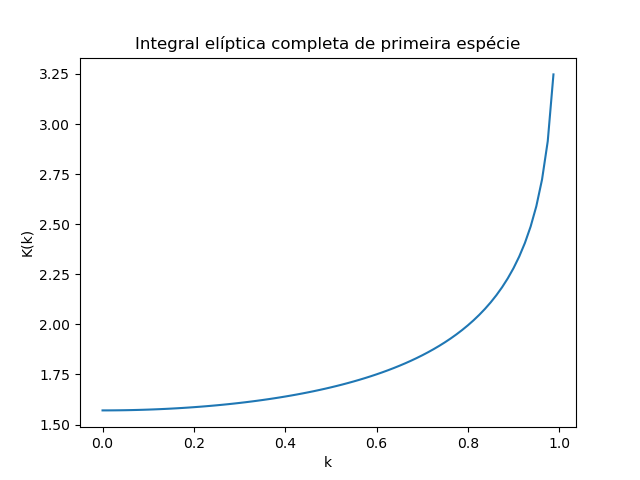
\includegraphics[scale=0.5]{Eliptica.png}
 \end{center}
 \caption{Integral elíptica completa de primeira espécie.}
 \label{Figura3}
\end{figure}

A figura (\ref{Figura3}) exibe um gráfico do comportamento da integral elíptica completa de primeira espécie $K(k)$, onde $0.0 \leq k=\sin{\left( \frac{\theta_0}{2} \right)} \leq 1.0$ e $0.0 \leq \theta_0 \leq \pi$. Este gráfico foi gerado utilizando o código (\ref{lista1}) em Python abaixo:

\lstinputlisting[caption=Resultados para a integral eliptica $K(k^2)$ como em (\ref{equa46}).,label=lista1]{eliptica.py}
 
Se estivermos interessados em determinar o período de oscilação devemos lembrar que ele é quatro vezes o intervalo de tempo para ir de $\theta=0$ a $\theta=\theta_0$ e analisando a expressão (\ref{equa48}):
\begin{eqnarray}
T & = & 4\, t(0\rightarrow \theta_0) \nonumber \\
& = & 4 \frac{\tau(0\rightarrow \theta_0)}{w_0} \nonumber \\
T & = & \frac{4}{w_0}\, K\left( \sin^2{\left( \frac{\theta_0}{2} \right) }\right),
 \label{equa53}
\end{eqnarray}
que mostra explicitamente a dependência do período de oscilação com a amplitude inicial $\theta_0$.

A figura (\ref{Figura4}) foi obtida utilizando o código (\ref{lista2}) em Python exibido na listagem abaixo, além disso, exibe os dois casos estudados até aqui. As curvas exibem dois comportamentos completamente distintos e evidencia a situação como a solução geral se contrapõe à solução para pequenas oscilações: é possível perceber que as duas curvas se sobrepõem entre $0.0 \leq \sin{(\frac{\theta_0}{2} )} \leq 0.1$. Além disso:

\begin{itemize}
 \item a curva azul representa a solução da equação diferencial não linear geral, ou seja, o período de oscilação do pêndulo varia com a amplitude inicial $0 \leq \theta_0 \leq \pi$ como na expressão (\ref{equa53});
 \item a curva laranja representa a solução particular para pequenas oscilações como na expressão (\ref{equa7}), ou seja, $\sin{(\theta)} \approx \theta$. 
\end{itemize}

Agora vamos mostrar alguns resultados de como $\theta(t)$, como em (\ref{equa18}) e (\ref{equa52}), se comporta em função de alguns valores de $\theta_0$. Vamos assumir que $w_0=\sqrt{2}s^{-1}$, como na nona linha do código (\ref{lista2}). Nos gráficos abaixo: as linhas na cor laranja representam resultados se fossem considerada solução tipo oscilador harmônico como em  (\ref{equa18}), as linhas na cor azul representam resultados envolvendo a solução geral (\ref{equa52}). O código (\ref{lista3}) foi utilizado para gerar os gráficos, para os vários valores de $\theta_0 = 0.01\pi, 0.1\pi, 0.25\pi, 0.50\pi, 0.75\pi \, \, \mbox{e} \, \, 0.90\pi$ que, para cada gráfico, deve ser substituído na sétima linha deste  código.

\begin{figure}
 \begin{center}
  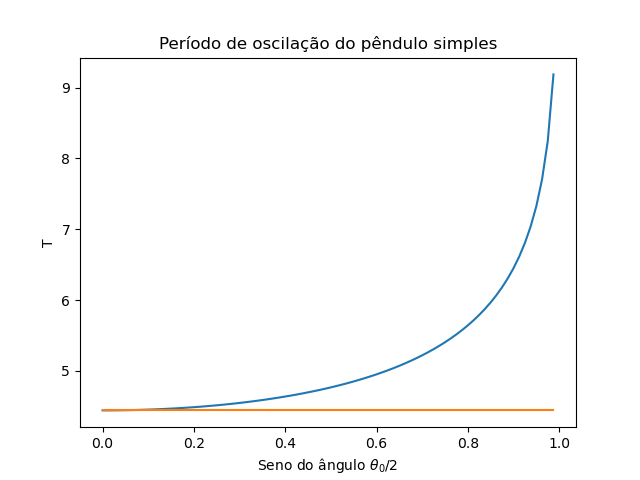
\includegraphics[scale=0.5]{Periodo.png}
 \end{center}
 \caption{Período de oscilação do pêndulo simples. Linha azul solução geral, linha laranja solução para pequenas oscilações.}
 \label{Figura4}
\end{figure}

\lstinputlisting[caption=Determina período de oscilação de acordo com as equações (\ref{equa7}) e (\ref{equa53}).,label=lista2]{periodo.py}

Nas figuras \ref{Figura5}, \ref{Figura6} e \ref{Figura7} (a,b) abaixo as curvas em azul exibem o comportamento para valores pequenos, médios e grandes do deslocamento angular inicial ($\theta_0$) (\ref{equa52}), respectivamente. As curvas em laranja são para o caso de pequenas oscilações (\ref{equa18}) apenas para efeito de comparação. Assim, estas figuras complementam o comportamento observado nos gráficos da figura \ref{Figura4} para o período de oscilação. Podemos observar que ao longo do tempo as curvas na cor azul e laranja divergem mais acentuadamente com o aumento de $\theta_0$. Por isso, a aproximação de pequenas oscilações ser a solução mais simples para o problema.

\lstinputlisting[caption=Como o ângulo $\theta(t)$ varia para cada situação inicial $\theta_0$ (pode variar na sétima linha).,label=lista3]{theta-tempo.py}

É possível escrever um código (\ref{lista4}) em Python, listagem abaixo, exibindo todas as curvas em um único gráfico. Contudo a análise fica mais complicada quando várias curvas estão presentes no mesmo gráfico vide figura \ref{Figura8}. O interesse aqui não é na exibição das curvas em si - consistindo um caso onde aquela máxima popular que diz: \textit{menos é mais} é fato - mas demonstrar a facilidade com que as contas podem ser feitas com a utilização do Python.
\vspace{1.0cm}

\begin{figure}[h]
 \centering
 \begin{subfigure}{.5\textwidth}
  \centering
  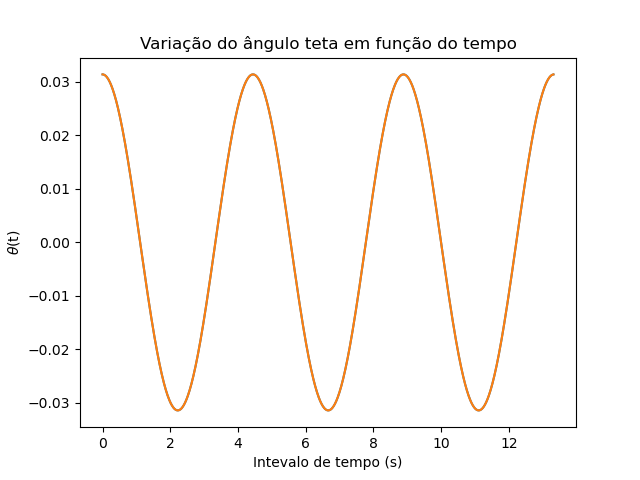
\includegraphics[width=1.1\linewidth]{teta-0-01pi.png}
  \caption{Considerando $\theta_0=0.01\pi$.}
  %\label{Figura5}
 \end{subfigure}%
 \begin{subfigure}{.5\textwidth}
  \centering
  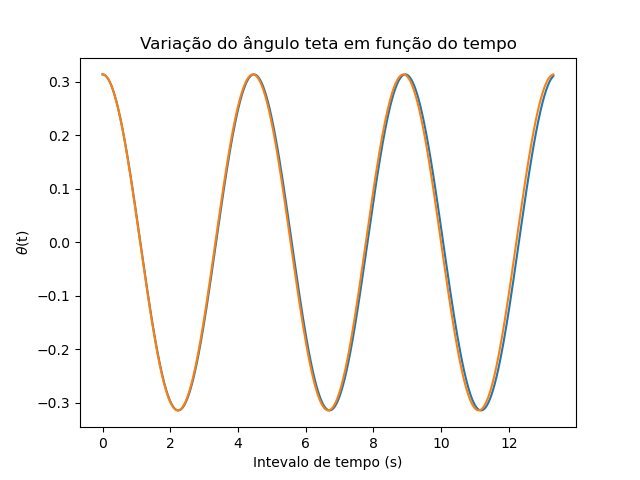
\includegraphics[width=1.1\linewidth]{teta-0-10pi.png}
  \caption{Considerando $\theta_0=0.10\pi$.}
  %\label{Figura6}
 \end{subfigure}
 \caption{Pequenos valores para o deslocamento angular inicial ($\theta_0$).}
 \label{Figura5}
\end{figure}

\begin{figure}[h]
 \centering
 \begin{subfigure}{.5\textwidth}
  \centering
  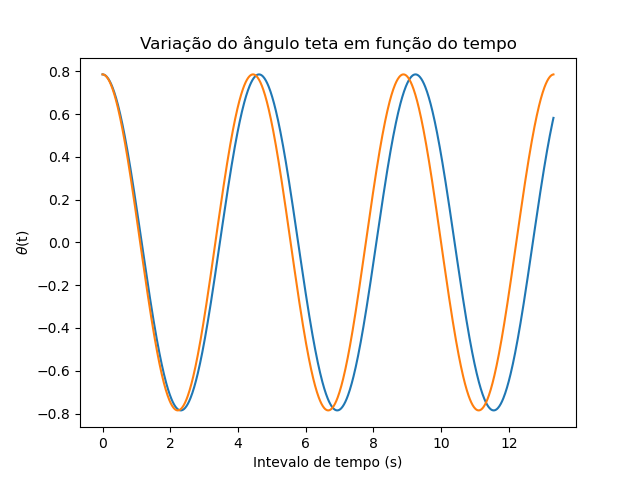
\includegraphics[width=1.1\linewidth]{teta-0-25pi.png}
  \caption{Considerando $\theta_0=0.25\pi$.}
  %\label{Figura7}
 \end{subfigure}%
 \begin{subfigure}{.5\textwidth}
  \centering
  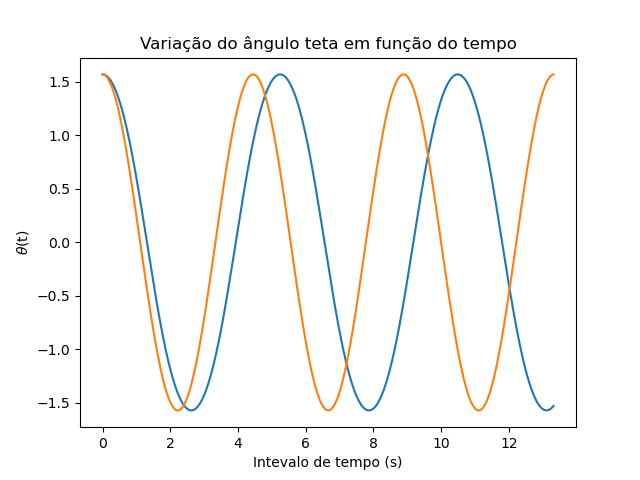
\includegraphics[width=1.1\linewidth]{teta-0-50pi.png}
  \caption{Considerando $\theta_0=0.50\pi$.}
  %\label{Figura8}
 \end{subfigure}
 \caption{Valores médios para o deslocamento angular inicial ($\theta_0$).}
 \label{Figura6}
\end{figure}

\begin{figure}[h]
 \centering
 \begin{subfigure}{.5\textwidth}
  \centering
  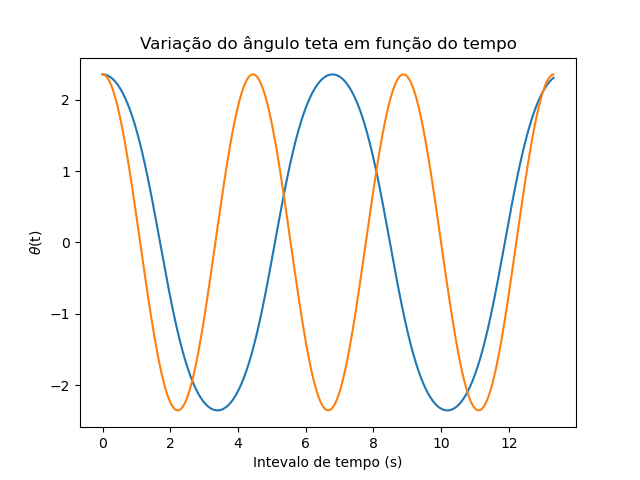
\includegraphics[width=1.1\linewidth]{teta-0-75pi.png}
  \caption{Considerando $\theta_0=0.75\pi$.}
  %\label{Figura9}
 \end{subfigure}%
 \begin{subfigure}{.5\textwidth}
  \centering
  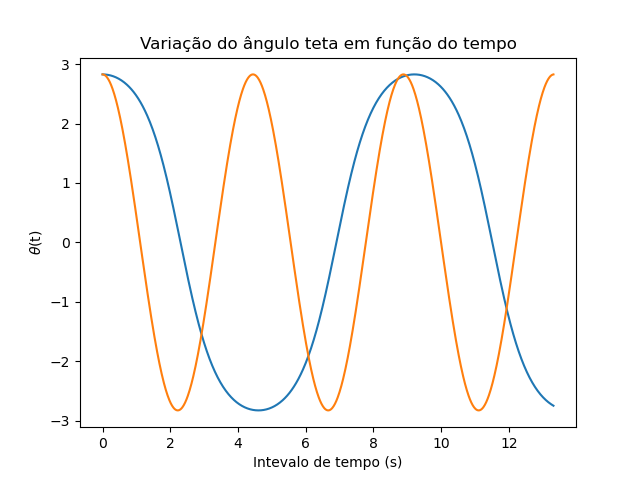
\includegraphics[width=1.1\linewidth]{teta-0-90pi.png}
  \caption{Considerando $\theta_0=0.90\pi$.}
  %\label{Figura10}
 \end{subfigure}
 \caption{Grandes valores para o deslocamento angular inicial ($\theta_0$).}
 \label{Figura7}
\end{figure}

\lstinputlisting[caption=Criando um gráfico com todas as situações das figuras (\ref{Figura5}) a (\ref{Figura7}).,label=lista4]{theta-tudo-tempo-sn.py}

\begin{figure}[h]
 \centering
 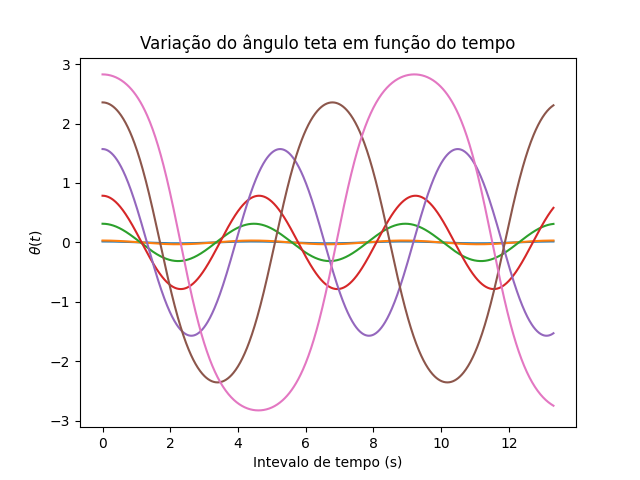
\includegraphics[width=1.0\linewidth]{teta-tudo.png}
 \caption{Comportamento de $\theta(t)$, para pequenas oscilações (laranja) e os valores: $0.01\pi$ (azul) meio misturada com a curva anterior, $0.10\pi$ (verde), $0.25\pi$ (vermelho), $0.50\pi$ (roxo), $0.75\pi$ (marrom) e $0.90\pi$ (rosa).}
 \label{Figura8}
\end{figure}


\section{Solução exata para velocidade inicial não nula}
A situação agora possui condições inciais distintas do caso anterior. Agora temos:
\begin{eqnarray}
 \theta_0 & = & 0, \nonumber \\
 & \mbox{e} & \nonumber \\
 v_0  = l \dot{\theta_0} & \neq & 0. \nonumber
\end{eqnarray}

A energia total do sistema em qualquer instante pode ser escrita como:
\begin{equation}
 E = K + U = \frac{1}{2} m v^2 + mgl \left[ 1 - \cos{(\theta)} \right] = \frac{1}{2} m v^2 + 2mgl \sin^2{\left( \frac{\theta}{2} \right)},
 \label{equa54}
\end{equation}
nas situações limites:
\begin{itemize}
 \item $\theta(t=0)=0$ e $v(t=0)=v_0$, ou seja no início do movimento na parte baixa, temos:
       \begin{equation}
        E(t=0) = \frac{1}{2}m v_0^2 
        \label{equa55}
       \end{equation}
 \item $\theta(t=T/4)=\theta_{max}$ e $v(t=T/4)=0$, ou seja em uma das extremidades do movimento, temos:
       \begin{equation}
        E(t=T/4) = mgl \left[ 1 - \cos{(\theta_{max})} \right] = 2 mgl \sin^2{\left( \frac{\theta_{max}}{2} \right) }.
        \label{equa56}
       \end{equation}
\end{itemize}

Igualando as duas expressões acima (\ref{equa55}) e (\ref{equa56}) teremos uma relação entre a velocidade inicial e o deslocamento angular máximo que o pêndulo pode sofrer:
\begin{eqnarray}
 v_0^2 & = & 4gl \sin^2{\left( \frac{\theta_{max}}{2} \right)} \nonumber \\
 \left( l \dot{\theta_0}\right)^2 & = & 4gl \sin^2{\left( \frac{\theta_{max}}{2} \right)} \nonumber \\
 \dot{\theta_0}^2 & = & 4 \frac{g}{l} \sin^2{\left( \frac{\theta_{max}}{2} \right)} = 4 w_0^2 \sin^2{\left( \frac{\theta_{max}}{2} \right)} \nonumber \\
 \dot{\theta_0} & = & 2w_0 \sin{\left( \frac{\theta_{max}}{2} \right)} \nonumber
\end{eqnarray}
assim:
\begin{eqnarray}
 \boxed{\theta_{max} = 2 \arcsin{\left( \frac{\dot{\theta_0}}{2w_0} \right)} = 2 \arcsin{\left( \frac{v_0}{2w_0 l} \right)} = 2 \arcsin{\left( \frac{v_0}{2\sqrt{gl}}\right)}}.
 \label{equa57}
\end{eqnarray}


Igualando as expressões (\ref{equa54}) e (\ref{equa56}) temos:
\begin{eqnarray}
 v^2 = (l \dot{\theta})^2 & = & 4gl \left[ \sin^2{\left( \frac{\theta_{max}}{2} \right)} - \sin^2{\left( \frac{\theta}{2} \right)} \right] \nonumber \\
 \dot{\theta}^2 & = & 4 w_0^2 \left[ \sin^2{\left( \frac{\theta_{max}}{2} \right)} - \sin^2{\left( \frac{\theta}{2} \right)} \right] \nonumber \\
 \frac{d\theta}{dt} & = & 2w_0 \sqrt{\sin^2{\left( \frac{\theta_{max}}{2} \right)} - \sin^2{\left( \frac{\theta}{2} \right)}}
\end{eqnarray}
ou:
\begin{eqnarray}
 w_0\, dt & = & \frac{1}{2} \frac{d\theta}{\sqrt{\sin^2{\left( \frac{\theta_{max}}{2} \right)} - \sin^2{\left( \frac{\theta}{2} \right)}}}, \nonumber
\end{eqnarray}
integrando a expressão acima teremos:
\begin{eqnarray}
 w_0t = \frac{1}{2} \int_0^{\theta} \frac{d\phi}{\sqrt{\sin^2{\left( \frac{\theta_{max}}{2} \right)} - \sin^2{\left( \frac{\phi}{2} \right)}}},
\end{eqnarray}
fazendo:
\begin{equation}
 k = \sin{\left( \frac{\theta_{max}}{2} \right)},
 \label{equa60}
\end{equation}
teremos:
\begin{eqnarray}
 w_0t = \frac{1}{2k} \int_0^{\theta} \frac{d\phi}{\sqrt{1 - \frac{1}{k^2} \sin^2{\left( \frac{\phi}{2} \right)}}}.
\end{eqnarray}

Por outro lado, se fizermos:
\begin{eqnarray}
 u = \frac{1}{k} \sin{\left( \frac{\phi}{2} \right)} & \rightarrow & du = \frac{1}{2k} \cos{\left( \frac{\phi}{2} \right)}\, d\phi,
\end{eqnarray}
assim:
\begin{eqnarray}
 d\phi = \frac{2k}{\cos{\left( \frac{\phi}{2} \right)}} du = \frac{2k}{\sqrt{1-\sin^2{\left( \frac{\phi}{2} \right)}}} du = \frac{2k}{\sqrt{1-k^2 u^2}} du,
\end{eqnarray}
portanto:
\begin{eqnarray}
 w_0t = \int_0^z \frac{du}{\sqrt{(1-k^2 u^2)(1-u^2)}} = F(\arcsin{(z)},k^2),
 \label{equa64}
\end{eqnarray}
que é a função elíptica incompleta de primeira ordem, com $z$ sendo o limite superior de $u$ quando $\phi=\theta$, ou:
\begin{equation}
 z = \frac{1}{k} \sin{\left( \frac{\theta}{2} \right)}.
\end{equation}
A inversa de (\ref{equa64}) é:
\begin{eqnarray}
 \arcsin{(z)} = am(w_0t,k^2) & \rightarrow & z = \sin{\left[ am(w_0t,k^2) \right]} \nonumber \\
 \frac{1}{k} \sin{\left( \frac{\theta}{2} \right)} & = & sn \left[ w_0t, k^2\right] \nonumber \\
 \sin{\left( \frac{\theta}{2} \right)} & = & \sin{\left( \frac{\theta_{max}}{2} \right)} sn \left[ w_0t, \sin^2{\left( \frac{\theta_{max}}{s} \right)} \right] \nonumber
\end{eqnarray}
após usar (\ref{equa60}), consequentemente:
\begin{eqnarray}
 \boxed{\theta(t) = 2 \arcsin{\left\{ \sin{\left( \frac{\theta_{max}}{2} \right)} sn \left[ w_0t, \sin^2{\left( \frac{\theta_{max}}{s} \right)} \right] \right\}}},
 \label{equa66}
\end{eqnarray}
é uma função do tempo dependendo das condições iniciais com $\theta_{max}$ obtido da expressão (\ref{equa57}) que depende da velocidade inicial $v_0$, da aceleração da gravidade $g$ e do comprimento do pêndulo.

Com relação ao período de oscilação do pêndulo nestas condições a expressão (\ref{equa53}) continua valendo mas com $\theta_0$ identificado como $\theta_{max}$ obtido pela expressão (\ref{equa60}). Assim sendo, $k\leq 1$, comparando a expressão (\ref{equa57}) com a (\ref{equa60}) temos a condição:
\begin{equation}
 \boxed{k = \frac{v_0}{2w_0l} \leq 1 \rightarrow v_0 \leq 2w_0l = 2\sqrt{gl}},
 \label{equa67}
\end{equation}
o que significa afirmar que o a velocidade inicial máxima depende do local (valor de $g$) e do comprimento $l$ do pêndulo.


Para completar nosso estudo sobre esta situação envolvendo as condições iniciais vamos fazer gráficos envolvendo a expressão (\ref{equa66}). Vamos utilizar o mesmo valor para $w_0=\sqrt{2} s^{-1}$ que na situação descrita na subseção anterior, a velocidade inicial está limitada como exibido na expressão (\ref{equa67}). O código (\ref{lista5}) baixo em Python cria os gráficos para serem analisados.

As curvas da figura \ref{Figura9} abaixo exibem o comportamento de $\theta(t)$ considerando três velocidades iniciais $v_0=w_0l$, $v_0=1.5\, w_0l$, $v_0=1.9\, w_0l$ e $v_0=1.999\, w_0l$. Observando as curvas é fácil perceber que à medida que $v_0$ aumenta da mesma forma temos um incremento da amplitude do movimento e consequentemente do período de oscilação do pêndulo.

\lstinputlisting[caption=Criando de uma só vez todos os gráficos segundo a equação (\ref{equa66}).,label=lista5]{theta-tempo-2-tudo.py}

\begin{figure}[t]
 \centering
 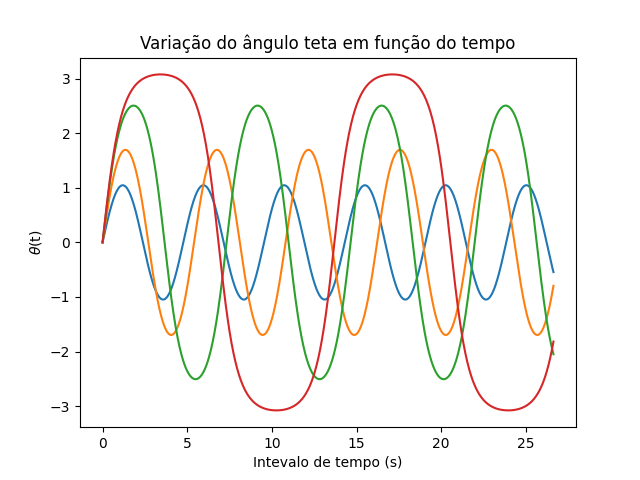
\includegraphics[width=1.0\linewidth]{teta-tudo-2.png}
 \caption{Comportamento de $\theta(t)$, para $v_0=w_0l$ (curva azul), $v_0=1.5\, w_0l$ (curva laranja), $v_0=1.9\, w_0l$ (curva verde) e $v_0=1.999\, w_0l$ (curva vermelha).}
 \label{Figura9}
\end{figure}

\chapter[O pêndulo simples amortecido]{O pêndulo simples amortecido}
\lettrine[nindent=0.35em,lhang=0.40,loversize=0.3]{A}{s} oscilações que estudamos na seção anterior ocorrem em sistemas conservativos. Em situações práticas sempre existe dissipação de energia. Toda vez que um sistema físico é posto a oscilar livremente, as oscilações decaem com o tempo até desaparecerem.

No caso particular do pêndulo, as oscilações são amortecidas devido à ação da resistência do ar. A contribuição do amortecimento, com $b$ sendo a constante de amortecimento, no processo é dada pelo arraste escrito aqui em termos da energia por intervalo de tempo (ou potência):
\begin{equation}
 F_a = \frac{b}{2} v^2 = \frac{b}{2} \, l^2 \dot{\theta}^2, \nonumber 
\end{equation}
que é proporcional ao quadrado da velocidade, as unidade da constante de amortecimento $b$ é $kg/s$, sendo a velocidade escrita na forma $v=l\frac{d \theta}{dt}=l\dot{\theta}$, e esta contribuição se opõe ao movimento do pêndulo.

A equação de Euler-Lagrange inicial \ref{equa2} pode ser reescrita para dar conta desta contribuição de amortecimento da seguinte forma:

\begin{eqnarray}
 \frac{d}{dt} \left( \frac{\partial L}{\partial \dot{\theta}} \right) - \frac{\partial L}{\partial \theta} = -\frac{\partial F_a}{\partial \dot{\theta}}.
 \label{equa68}
\end{eqnarray}

Assim, a equação diferencial homogênea geral que descreve o pêndulo simples amortecido com constante de amortecimento $b$ pode ser escrita como:
\begin{eqnarray}
 m\, l^2\ddot{\theta} + b\, l^2\, \dot{\theta} + m\, g \, l \sin{(\theta)} & = & 0 \nonumber \\
 \ddot{\theta} + \frac{b}{m} \dot{\theta} + \frac{g}{l} \sin{(\theta)} & = & 0.
 \label{equa69}
\end{eqnarray}
Que, quando comparada à equação \ref{equa3}, surge um termo adicional que complica um pouco mais a solução geral. Se lembrarmos que $w_0^2=\frac{g}{l}$ e fizermos $\gamma = \frac{b}{m}$ teremos:
\begin{eqnarray}
 \ddot{\theta} + \gamma \, \dot{\theta} + w_0^2 \, \sin{(\theta)} & = & 0.
 \label{equa70}   
\end{eqnarray}
A questão agora se resume na solução da equação diferencial de segunda ordem acima \ref{equa70}. Vamos abordar esta equação diferencial envolvendo inicialmente pequenas oscilações e a seguir buscar uma solução geral.

\section{Pequenas oscilações}
A equação diferencial \ref{equa70}, ao meu conhecimento, só possui solução analítica para pequenas oscilações, ou seja $\sin{(\theta)} \approx \theta$, assim a equação diferencial \ref{equa70} toma a forma:
\begin{eqnarray}
 \ddot{\theta} + \gamma \, \dot{\theta} + w_0^2 \, \theta & = & 0.
 \label{equa71}   
\end{eqnarray}
De início, vamos transformar a equação diferencial acima num sistema de equações diferenciais através de uma mudança de variável:
\begin{eqnarray}
 \dot{\theta} & = & \Omega \nonumber \\
 \dot{\Omega} & = & - \gamma \, \Omega - w_0^2 \, \theta
 \label{equa72}
 \end{eqnarray}
que permite a introdução de duas equações diferenciais acopladas e que podem ser reescritas da seguinte forma:
\begin{eqnarray}
 \frac{d}{dt} \begin{bmatrix}
                \theta \\
                \Omega
                \end{bmatrix} & = & \begin{bmatrix}
                                      0 & 1 \\
                                      -w_0^2 & -\gamma
                                    \end{bmatrix}
                                    \begin{bmatrix}
                                      \theta \\
                                      \Omega                  
                                    \end{bmatrix},
 \label{equa73}
\end{eqnarray}
o plano formado por $\theta$ e $\Omega$ é denominado de plano de fase e um conjunto de trajetórias neste plano é designado de retrato de fase.

Desta forma, se identificarmos
\begin{eqnarray}
 \mathbb{X}(t) = \begin{bmatrix}
          \theta(t) \\
          \Omega(t)
         \end{bmatrix},
 \label{equa74}
\end{eqnarray}
as condições iniciais escritas como:
\begin{eqnarray}
 \mathbb{X}_0(t=t_0) = \begin{bmatrix}
             \theta_0 \\
             \Omega_0
            \end{bmatrix}, \nonumber
\end{eqnarray}
e a matriz:
\begin{eqnarray}
 \mathbb{A} = \begin{bmatrix}
      0 & 1 \\
      -w_0^2 & -\gamma
      \end{bmatrix},
 \label{equa75}
\end{eqnarray}
pelo fato do determinante desta matriz ser diferente de zero ela é invertível.  Além disso, o processo de diagonalização da matriz $\mathbb{A}$ nos leva a escrevê-la na forma:
\begin{equation}
 \mathbb{A} = \mathbb{P}\, \mathbb{D}\, \mathbb{P}^{-1}
 \label{equa76}
\end{equation}
onde $\mathbb{P}$ é a matriz de autovetores da matriz $\mathbb{A}$:
\begin{equation}
 \mathbb{P} = \begin{bmatrix}
      V & Z
      \end{bmatrix} = \begin{bmatrix}
                       v_1 & z_1 \\
                       v_2 & z_2
                      \end{bmatrix},
 \label{equa77}
\end{equation}
e $\mathbb{D}$ a matriz de autovalores da matriz $\mathbb{A}$:
\begin{equation}
 \mathbb{D} = \begin{bmatrix}
      \lambda_1 & 0 \\
      0 & \lambda_2
     \end{bmatrix}.
 \label{equa78}
\end{equation}


Além disso, o problema de valor inicial que estamos tentando resolver toma a forma:
\begin{equation}
 \begin{cases}
  \frac{d}{dt}\mathbb{X}(t) & =  \mathbb{X}'(t) =  \mathbb{A}\, \mathbb{X}(t) \\
  \mathbb{X}(t_0) & = \mathbb{X}_0.
 \end{cases}
 \label{equa79}
\end{equation}

A equação característica deste problema pode ser obtida da solução do seguinte determinante:
\begin{eqnarray}
 \begin{vmatrix}
  -\lambda & 1 \\
  -w_0^2 & -\gamma -\lambda
 \end{vmatrix} & = & 0
 \label{equa80} 
\end{eqnarray}
com a forma:
\begin{eqnarray}
 \lambda\, (\gamma + \lambda) + w_0^2 & = & 0 \nonumber \\
 \lambda^2 + \gamma\, \lambda + w_0^2 & = & 0
 \label{equa81}
\end{eqnarray}
tal que as raízes (autovalores) são:
\begin{equation}
 \begin{cases}
   \lambda_1 & =  -\frac{\gamma}{2} - \sqrt{\frac{\gamma^2}{4} - w_0^2} = -\frac{\gamma}{2} - \beta, \\
   \lambda_2 & =  -\frac{\gamma}{2} + \sqrt{\frac{\gamma^2}{4} - w_0^2} = -\frac{\gamma}{2} + \beta.
 \end{cases}
 \label{equa82}
\end{equation}
Assim, a solução geral depende do sinal de $\left(\frac{\gamma^2}{4} - w_0^2 \right)$, sendo $\beta = \sqrt{\frac{\gamma^2}{4} - w_0^2}$. Além disso os autovetores associados aos autovalores \ref{equa82} são obtidos a partir de:
\begin{eqnarray}
 \begin{bmatrix}
 -\lambda & 1 \\
 -w_0^2 & -\gamma - \lambda
 \end{bmatrix} \begin{bmatrix}
                 u_1 \\
                 u_2
                \end{bmatrix} = 0,
 \label{equa83}
\end{eqnarray}
que nos leva a:
\begin{equation}
 \begin{cases}
  -\lambda \, u_1 + u_2 = 0 & \rightarrow \, \,  u_2 = \lambda \, u_1 \\
  -w_0^2 \, u_1 - (\gamma + \lambda) u_2 = 0 & \rightarrow \, \,  \text{ que nos leva a \ref{equa81} após substituir $u_2$}.
 \end{cases}
 \label{equa84}
\end{equation}
Consequentemente, uma vez que temos duas raízes, os autovetores que são solução geral são da forma:
\begin{eqnarray}
 \begin{cases}
  V & = \begin{bmatrix}
         v_1 \\
         \lambda_1 \, v_1
         \end{bmatrix} \\
    & \\
  Z & = \begin{bmatrix}
         z_1 \\
         \lambda_2 \, z_1
        \end{bmatrix}
 \end{cases}
 \label{equa85}     
\end{eqnarray}

\subsection{Amortecimento forte}
Nesta situação $\gamma^2 > 4 w_0^2$, as soluções do polinômio característico ($\lambda_1$ e $\lambda_2$) são reais, distintas e negativas já que $\beta < \frac{\gamma}{2}$. Então, quando $t\rightarrow \infty$ as soluções do problema devem convergem para zero e teremos um sistema estável. Assim, utilizando \ref{equa76}, a equação diferencial matricial em \ref{equa79} pode ser escrita como:
\begin{equation}
 \mathbb{X}'(t) = \mathbb{P}\, \mathbb{D}\, \mathbb{P}^{-1} \mathbb{X}(t),
 \label{equa86}
\end{equation}
multiplicando por $\mathbb{P}^{-1}$ teremos:
\begin{eqnarray}
 \mathbb{P}^{-1}\, \mathbb{X}'(t) & = & \mathbb{P}^{-1}\, \mathbb{P}\, \mathbb{D}\, \mathbb{P}^{-1}\, \mathbb{X}(t) \nonumber \\
                & = & \mathbb{D}\, \mathbb{P}^{-1}\, \mathbb{X}(t).
 \label{equa87}
\end{eqnarray}
Fazendo uma mudança de variável:
\begin{equation}
 \mathbb{Y}(t) = \mathbb{P}^{-1}\, \mathbb{X}(t) \rightarrow \mathbb{Y}'(t) = \mathbb{P}^{-1}\, \mathbb{X}'(t)
 \label{equa88}
\end{equation}
logo:
\begin{equation}
 \mathbb{Y}'(t) = \mathbb{D}\, \mathbb{Y}(t)\rightarrow \begin{bmatrix}
                              y'_1(t) \\
                              y'_2(t)
                              \end{bmatrix} = \begin{bmatrix}
                                               \lambda_1 & 0 \\
                                               0 & \lambda_2
                                               \end{bmatrix} \begin{bmatrix}
                                                y_1(t) \\
                                                y_2(t)
                                               \end{bmatrix}
 \label{equa89}
\end{equation}
que pode ser escrita como duas expressões desacopladas:
\begin{equation}
 \begin{cases}
  y'_1(t) = & \lambda_1 \, y_1(t) \rightarrow y_1(t) = A\, e^{\lambda_1\, t}, \\
  y'_2(t) = & \lambda_2 \, y_2(t) \rightarrow y_2(t) = B\, e^{\lambda_2\, t}.
 \end{cases}
 \label{equa90}
\end{equation}
Por outro lado:
\begin{equation}
 \mathbb{P}\, \mathbb{Y}(t) = \mathbb{P}\, \mathbb{P}^{-1}\, \mathbb{X}(t) \rightarrow \mathbb{X}(t) = \mathbb{P}\, \mathbb{Y}(t)
 \label{equa91}
\end{equation}
assim:
\begin{equation}
 \mathbb{X}(t) = \begin{bmatrix}
         v_1 & z_1 \\
         v_2 & z_2 \\
         \end{bmatrix} \begin{bmatrix}
                        A\, e^{\lambda_1\, t} \\
                        B\, e^{\lambda_2\, t}
                       \end{bmatrix} = A\, e^{\lambda_1\, t} \begin{bmatrix}
                        v_1 \\
                        v_2
                       \end{bmatrix} + B\, e^{\lambda_2\, t} \begin{bmatrix}
                        z_1 \\                                         
                        z_2
                       \end{bmatrix},
 \label{equa92}
\end{equation}
lembrando de \ref{equa85}:
\begin{equation}
 \mathbb{X}(t) = A\, e^{\lambda_1\, t} \begin{bmatrix}
                               v_1 \\
                               \lambda_1 \, v_1
                               \end{bmatrix} + B\,  e^{\lambda_2\, t}\begin{bmatrix}
                                z_1 \\
                                \lambda_2 \, z_1
                               \end{bmatrix}.
 \label{equa93}
\end{equation}

Consequentemente, considerando $v_1 = z_1 = 1$ e os autovalores \ref{equa82}, a solução geral do sistema \ref{equa73} pode ser identificada como:
\begin{equation}
 \begin{cases}
  \theta(t) & = e^{-\gamma \, t/2} \left[ A\, e^{-\beta\, t} + B\, e^{\beta\, t} \right], \\
  \Omega(t) & = e^{-\gamma \, t/2} \left[ C\, e^{-\beta\, t} + D\, e^{\beta\, t} \right],
 \end{cases}
 \label{equa94}
\end{equation}
com $A$, $B$, $C=A\, \lambda_1$ e $D=B\, \lambda_2$ determinadas pelas condições iniciais do problema:
\begin{eqnarray}
 \mathbb{X}_0(t=0) = \begin{bmatrix}
  \theta(t=0) \\
  \Omega(t=0)
  \end{bmatrix} = \begin{bmatrix}
                   \theta_0 \\
                   \Omega_0
                 \end{bmatrix},
 \label{equa95}
\end{eqnarray}
que nos leva a:
\begin{eqnarray}
 A + B & = & \theta_0 \nonumber \\
 A\, \lambda_1 + B\, \lambda_2 & = & \Omega_0, \nonumber
\end{eqnarray}
resumindo:
\begin{eqnarray}
 A = \frac{\theta_0\, \lambda_2 - \Omega_0}{\lambda_2 - \lambda_1} & \text{e} & B = \frac{\Omega_0 - \theta_0\, \lambda_1}{\lambda_2 - \lambda_1}.
 \label{equa96}
\end{eqnarray}

As figuras \ref{Figura10} e \ref{Figura11} foram geradas utilizando o código Python listado abaixo. Substituindo o valor de gama (na linha 12 do código) por $3.0\, w_0$ (referente à figura \ref{Figura10}) ou $5.0 w_0$ (referente à figura \ref{Figura11}), respectivamente. Além disso as condições iniciais levam em consideração que a posição inicial é $\theta_0=0.1$ (linha 18 do código) e três valores para a velocidade inicial $\Omega_0=(0.0,0.5,-0.5)s^{-1}$ (linha 20 do código). Podemos verificar no código que o comprimento do pêndulo e o local onde o experimento é realizado são os mesmos das situações sem amortecimento.

\lstinputlisting{amortecido-forte.py}

Observando as figuras \ref{Figura10} e \ref{Figura11} percebemos que quando $\gamma$ aumenta o sistema, para as mesmas condições iniciais, demora mais tempo para entrar em repouso.
    
\begin{figure}[h]
 \centering
 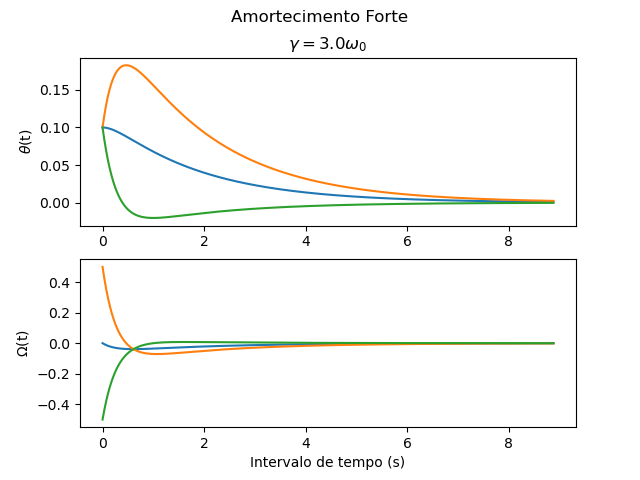
\includegraphics[width=1.0\linewidth]{forte-1.png}
 \caption{Comportamento de $\theta(t)$ - gráfico superior - e $\Omega(t)$ - gráfico inferior no caso em que $\gamma = 3.0\,  w_0$, para $\Omega_0=0$ (curva azul), $\Omega_0=0.5 s^{-1}$ (curva laranja) e $\Omega_0=-0.5 s^{-1}$ (curva verde).}
 \label{Figura10}
\end{figure}

No caso em que a velocidade inicial é nula, a posição do corpo diminui monotonamente em direção à zero. No caso de velocidade inicial positiva a posição angular é aumentada, atingindo um máximo começando a diminuir até atingir a sua
posição natural. No caso da velocidade inicial ser negativa, a posição angular é diminuída, empurrando a massa m e o movimento vai decaindo monotonamente até à sua posição final nula.

\begin{figure}[h]
 \centering
 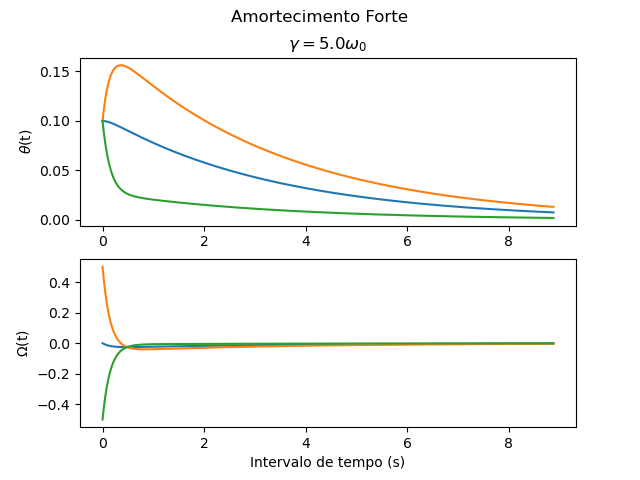
\includegraphics[width=1.0\linewidth]{forte-2.png}
 \caption{Comportamento de $\theta(t)$ - gráfico superior - e $\Omega(t)$ - gráfico inferior no caso em que $\gamma = 5.0\,  w_0$, para $\Omega_0=0$ (curva azul), $\Omega_0=0.5 s^{-1}$ (curva laranja) e $\Omega_0=-0.5 s^{-1}$ (curva verde).}
 \label{Figura11}
\end{figure}

A figura \ref{Figura12} foi obtida utilizando o código Python abaixo. Esta figura exibe o comportamento do sistema a partir das condições iniciais $\theta_0=0$ e $\Omega_0=0.5s^{-1}$ para o caso em que $\gamma=3.0\, w_0$. No gráfico do espaço de fase a distância entre um ponto e outro é da ordem de $8,9\times 10^{-3}s$.

\lstinputlisting{fase-forte.py}

\begin{figure}[t]
 \centering
 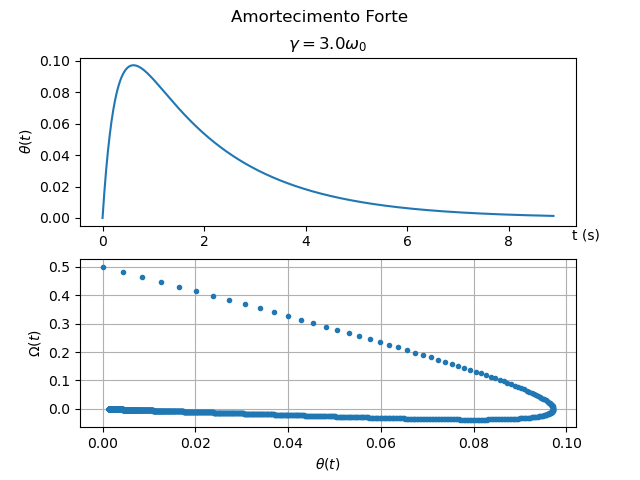
\includegraphics[width=1.0\linewidth]{forte-fase-1.png}
 \caption{Comportamento $\theta(t)$ e do espaço de fase $\Omega(t)$ contra $\theta(t)$ para o caso em que $\gamma=3.0\, w_0$, ou seja amortecimento forte, e as seguintes condições iniciais $\theta_0=0$ e $\Omega_0=0.5s^{-1}$.}
 \label{Figura12}
\end{figure}


\subsection{Amortecimento crítico}
Nesta situação $\gamma^2 = 4\, w_0^2 \rightarrow \beta = 0$ assim segundo \ref{equa82} temos que $\lambda_1=\lambda_2 = \lambda = -\frac{\gamma}{2}$.Assim, as soluções (autovetores) para este autovalor são degenerados, então devemos tomar cuidado. Aqui temos uma diferença importante, escreveremos a matriz $\mathbb{A}$ como:
\begin{equation}
 \mathbb{A} = \mathbb{P}\, \mathbb{J}\, \mathbb{P}^{-1},
 \label{equa97}
\end{equation}
onde $\mathbb{J}$ é a matriz de Jordan e pode ser escrita da forma:
\begin{equation}
 \mathbb{J} = \begin{bmatrix}
               \lambda & 1 \\
               0 & \lambda
              \end{bmatrix}.
 \label{equa98}
\end{equation}
Assim, semelhante a \ref{equa89}:
\begin{equation}
 \mathbb{Y}'(t) = \mathbb{J}\, \mathbb{Y}(t) = \begin{bmatrix}
                     \lambda & 1 \\
                     0 & \lambda
                     \end{bmatrix} \begin{bmatrix}
                                    y_1(t) \\
                                    y_2(t)
                                   \end{bmatrix},
 \label{equa99}
\end{equation}
que, escrevendo na forma de um sistema de equações, nos leva a:
\begin{equation}
 \begin{cases}
 y'_1(t) = & \lambda\, y_1(t) + y_2(t) \\
 y'_2(t) = & \lambda\, y_2(t)
 \end{cases} \rightarrow \begin{cases}
                          y'_1(t) = & \lambda\, y_1(t) + B\, e^{\lambda\, t} \\
                          y_2(t) = & B\, e^{\lambda\, t}
                         \end{cases},
 \label{equa100}
\end{equation}
para resolver a primeira equação precisamos encontrar uma função $y_1(t)$ que não seja um múltiplo de $y_2(t)$. Vamos considerar então a primeira solução, fazendo $B=1$ como: $y_2(t) = e^{-\frac{\gamma}{2} t}$, e a segunda solução linearmente independente como:
\begin{equation}
 y_1(t) = u(t)\, e^{-\frac{\gamma}{2} t},
 \label{equa101}
\end{equation}
logo:
\begin{equation}
 \begin{cases}
y'_1(t) & = u'(t)\, e^{-\frac{\gamma}{2} t} - \frac{\gamma}{2} u(t)\, e^{-\frac{\gamma}{2}t}  = \left[ u'(t) - \frac{\gamma}{2} \, u(t) \right] e^{-\frac{\gamma}{2} t}, \\
y''_1(t) & = u''(t)\, e^{-\frac{\gamma}{2} t} - \gamma\, u'(t)\, e^{-\frac{\gamma}{2}t} + \left( \frac{\gamma}{2} \right)^2 \, u(t)\, e^{-\frac{\gamma}{2} t}  \\
& = \left[ u''(t) - \gamma\, u'(t) + \left( \frac{\gamma}{2} \right)^2\, u(t) \right] e^{-\frac{\gamma}{2} t},
 \end{cases}
 \label{equa102}
\end{equation}
substituindo \ref{equa101} e \ref{equa102} em \ref{equa71} e após eliminar $e^{-\frac{\gamma}{2} t}$ teremos:
\begin{eqnarray}
\left[ u''(t) - \gamma\, u'(t) + \left( \frac{\gamma}{2} \right)^2  \right] & + & \gamma \left[ u'(t) - \frac{\gamma}{2} \right] + w_0^2\, u(t) = 0 \nonumber \\
u''(t) & + & \left( \frac{\gamma^2}{4} - \frac{\gamma^2}{2} + w_0^2 \right) u(t) = 0 \nonumber \\
u''(t) & + & \left( -\frac{\gamma^2}{4} + w_0^2 \right) u(t) = 0 \nonumber \\
u''(t) = 0 &\rightarrow & u(t) = B\, t + A,
 \label{103}
\end{eqnarray}
consequentemente \ref{equa101} torna-se:
\begin{equation}
 y_1(t) = (B \, t + A)\, e^{\lambda\, t}.
 \label{equa104}
\end{equation}
Por outro lado:
\begin{eqnarray}
 \mathbb{X}(t) = \mathbb{P}\, \mathbb{Y}(t) & = & \begin{bmatrix}
                    v_1 & z_1 \\
                    v_2 & z_2 
                    \end{bmatrix} \begin{bmatrix}
                                   (A + B\, t) e^{\lambda\, t} \\
                                   B\, e^{\lambda\, t}
                                   \end{bmatrix} \nonumber \\
                 & = & (A + B\, t)\, e^{\lambda\, t} \begin{bmatrix}
                  v_1 \\
                  v_2
                  \end{bmatrix} + B\, e^{\lambda\, t} \begin{bmatrix}
                   z_1 \\
                   z_2
                  \end{bmatrix},
 \label{equa105}
\end{eqnarray}
ainda falta determinar os vetores $V$ e $Z$, ou seja a matriz $\mathbb{P}$. Se multiplicarmos a matriz $\mathbb{A}$ em \ref{equa97} à direita por $\mathbb{P}$ teremos:
\begin{eqnarray}
\mathbb{A}\, \mathbb{P} & = & \mathbb{P} \, \mathbb{J} \, \mathbb{P}^{-1} \, \mathbb{P} = \mathbb{P} \, \mathbb{J} \nonumber \\
\mathbb{A} \, \begin{bmatrix}
               V & Z
               \end{bmatrix} & = & \begin{bmatrix}
                                    V & Z
                                   \end{bmatrix} \mathbb{J} \nonumber \\
 \begin{bmatrix}
  \mathbb{A} \, V & \mathbb{A} \, Z
 \end{bmatrix} & = & \begin{bmatrix}
                      \lambda \, V & V + \lambda\, Z
                     \end{bmatrix},  \nonumber
\end{eqnarray}
comparando coluna a coluna:
\begin{equation}
 \begin{cases}
  \mathbb{A} \, V & = \lambda \, V \rightarrow (\mathbb{A} - \lambda \mathbb{I}) \, V = 0, \\
  \mathbb{A} \, Z & = V + \lambda \, Z \rightarrow (\mathbb{A} - \lambda \mathbb{I}) \, Z = V,
 \end{cases}
 \label{equa106}
\end{equation}
o que significa que após obtermos o vetor $V$ é possível obter o vetor $Z$ de forma simples.

 Um autovetor solução de \ref{equa79} é:
\begin{eqnarray}
 V & = & (v_1,\lambda v_1) \rightarrow \text{fazendo} \rightarrow v_1 = 1 \rightarrow V = (1,\lambda),
 \label{equa107}
\end{eqnarray}
o segundo vetor pode ser obtido através de:
\begin{eqnarray}
 \begin{bmatrix}
  -\lambda & 1 \\
  -w_0^2 & -\gamma -\lambda
  \end{bmatrix} \begin{bmatrix}
                 z_1 \\
                 z_2
                 \end{bmatrix} = \begin{bmatrix}
                                  1 \\
                                  \lambda
                                  \end{bmatrix},
 \label{equa108}
\end{eqnarray}
que nos leva a:
\begin{eqnarray}
 -\lambda\, z_1 + z_2 = 1 & \rightarrow & z_2 = 1 + \lambda \, z_1 \\
 -w_0^2 \, z_1 - (\gamma + \lambda) z_2 = \lambda & \rightarrow & \text{que quando substituído $z_2$ nos leva a $0=0$.} \nonumber
 \label{equa109} 
\end{eqnarray}
Assim, o segundo vetor é:
\begin{eqnarray}
 Z & = & (z_1,1+\lambda z_1) \rightarrow \text{fazendo} \rightarrow z_1 = 1 \rightarrow Z =(1,1+\lambda).
 \label{equa110}
\end{eqnarray}
Consequentemente, as soluções gerais para \ref{equa73} têm a forma:
\begin{equation}
 \mathbb{X}(t) = (A + B\, t)\, e^{\lambda\, t} \begin{bmatrix}
                                             1 \\
                                             \lambda
                                             \end{bmatrix} + B\, e^{\lambda\, t} \begin{bmatrix}
                                              1 \\
                                              1 + \lambda
                                             \end{bmatrix}
 \label{equa111}
\end{equation}
ou , de forma mais específica:
\begin{equation}
 \begin{cases}
 \theta(t) & = (A + B\, t)\,  e^{\lambda\, t} + B\, e^{\lambda \, t} = A_c \, e^{\lambda\, t} + B\, t\, e^{\lambda\, t} \\
 \Omega(t) & = \lambda\, (A + B\, t)\,  e^{\lambda \, t} + (1+\lambda)\, B \, e^{\lambda\, t} = C_c\, e^{\lambda\, t} + D\, t\, e^{\lambda\, t}
 \end{cases}
 \label{equa112}
\end{equation}
sendo $A_c = A + B$, $B$, $C_c=A_c\, \lambda+B$ e $D=B \lambda$ obtidos via condições iniciais do sistema em, digamos, $t=0$ $\theta(t=0)=\theta_0$ e $\Omega(t=0)=\Omega_0$, que nos leva a:
\begin{eqnarray}
 A_c & = & \theta_0 \nonumber \\
 A_c\, \lambda + B & = & \Omega_0, \nonumber
\end{eqnarray}
assim:
\begin{equation}
 \begin{cases}
  A_c = & \theta_0, \\
  B = & \Omega_0 - \lambda \, \theta_0.
 \end{cases}
 \label{equa113}
\end{equation}
Em decorrência:
\begin{equation}
 \begin{cases}
  C_c = A_c\, \lambda + B & =  \theta_0 \, \lambda + \Omega_0 - \lambda \, \theta_0 = \Omega_0, \\
  D = B\, \lambda & =  \Omega_0 \, \lambda - \theta_0 \, \lambda^2.
 \end{cases}
 \label{equa114}
\end{equation}

\lstinputlisting{amortecido-critico.py}

Tanto caso do movimento ser fortemente amortecido ou na situação em que temos um amortecimento crítico, a solução $\theta(t)$ tende a atingir a posição natural de equilíbrio com a passagem do tempo, independentemente das constantes $A$, $A_c$ e $B$.

\begin{figure}[t]
 \centering
 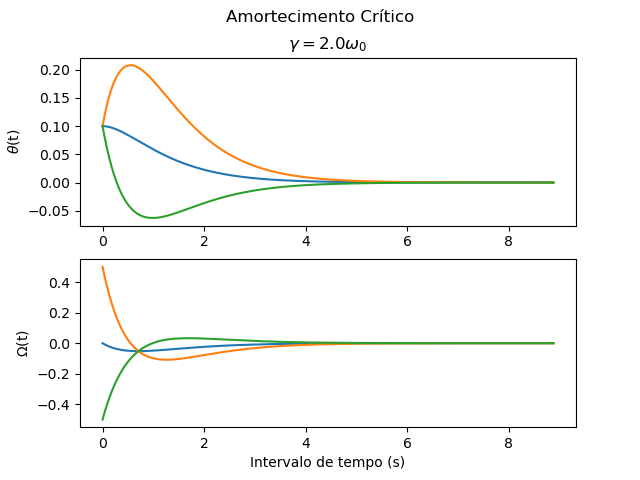
\includegraphics[width=1.0\linewidth]{critico-1.png}
 \caption{Comportamento $\theta(t)$ e da velocidade $\Omega(t)$ para o caso em que $\gamma=2.0\, w_0$, ou seja amortecimento crítico, e as seguintes condições iniciais $\theta_0=0.1$ e $\Omega_0=0.0$ (curva azul), $\Omega_0=0.5s^{-1}$ (curva laranja) e $\Omega_0=-0.5s^{-1}$ (curva verde).}
 \label{Figura13}
\end{figure}

\subsection{Amortecimento fraco}

\section{Oscilações genéricas}

\lstinputlisting{ODE-solutions.py}

\begin{figure}[t]
 \centering
 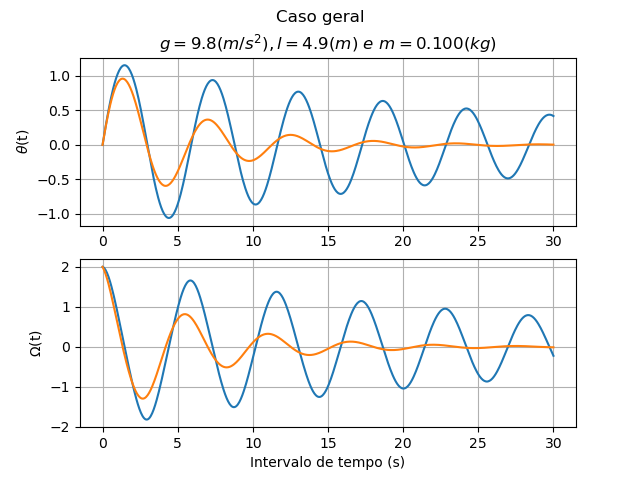
\includegraphics[width=1.0\linewidth]{caso-geral-1.png}
 \caption{Comportamento $\theta(t)$ e da velocidade $\Omega(t)$ para o caso em que, utilizando a expressão \ref{equa69}, temos $b=0.01\, kg/s$ (curva azul) e $b=0.05\, kg/s$ (curva laranja).}
 \label{Figura14}
\end{figure}

\lstinputlisting{ODE-solutions-fase.py}

\begin{figure}[t]
 \centering
 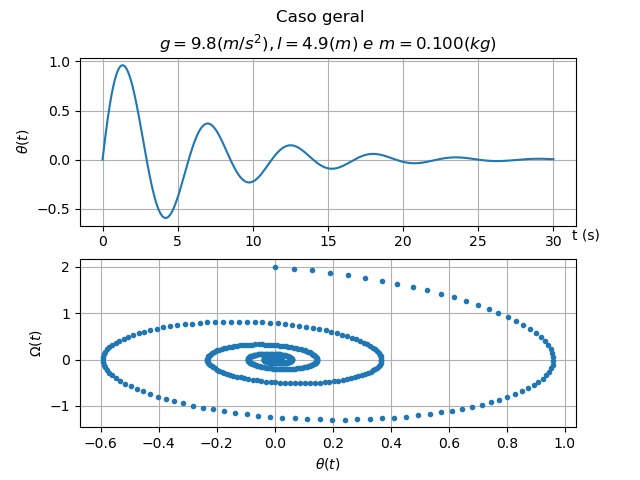
\includegraphics[width=1.0\linewidth]{caso-geral-2.png}
 \caption{Comportamento $\theta(t)$ e do espaço de faze velocidade $\Omega(t)$ contra $\theta(t)$ para o caso em que, utilizando a expressão \ref{equa69}, temos $b=0.05\, kg/s$.}
\label{Figura15}
\end{figure}

\postextual
\bibliography{livro-1}

\end{document}
